% !TEX root = ../main.tex

% 分析与讨论	
\begin{table}
	\renewcommand\arraystretch{1.7}
	\begin{tabularx}{\textwidth}{|X|X|X|X|}
		\hline
		Major:& Physics &Grade:& 2022\\
		\hline
		Name: & \textbf{杨舒云、戴鹏辉、朱政鑫、马万成} & Student number:& 22344020、22344016、22344019、22344018\\
		\hline
		Date:& 2024/10/18 & Score: &\\
		\hline
	\end{tabularx}
\end{table}
\section{APL1-3 氦氖激光综合实验 \\ Analysis \& Discussion}


%---------------------------------------------------------------------
% 数据处理
\subsection{Data Processing}

% 分析
\subsubsection{Analysis}
由杨舒云22344020主导,我们编写了Python脚本(代码见附件),完成了这部分数据处理。
\begin{enumerate}
	\item 高斯光束参数计算
	
	根据实验数据作图,并计算出光腰位置、光腰半径、瑞利长度、远场发散角。结果如\cref{tab:exp3-a-1}、\cref{tab:exp3-a-2}和\cref{fig:apl18exp3analysis}所示。
	
	\begin{table}[h!]
		\centering
		\renewcommand{\arraystretch}{1.5} % 调整行高
		\caption{Beam Parameters (from python script)}
		\label{tab:exp3-a-1}
		\begin{tabular}{|c|c|}
			\hline
			\textbf{Parameter} & \textbf{Value} \\ \hline
			Beam Waist Position ($z_0$) & 283.71 mm \\ \hline
			Beam Waist Radius ($\omega_0$) & 0.4617 mm \\ \hline
			Divergence Angle ($\theta$) & 0.002456 rad \\ \hline
			Rayleigh Length ($Z_0$) & 187.96 mm \\ \hline
		\end{tabular}
	\end{table}
	
	\begin{table}[h!]
		\centering
		\renewcommand{\arraystretch}{1.5} % 调整行高
		\caption{Beam Parameters (from the lab software)}
		\label{tab:exp3-a-2}
		\begin{tabular}{|c|c|c|c|c|c|}
			\hline
			\textbf{a/b 轴} & \textbf{远场发散角 (mrad)} & \textbf{光腰位置 (mm)} & \textbf{光腰半径 (mm)} & \textbf{瑞利长度 (mm)} & \textbf{M\textsuperscript{2} 因子} \\ \hline
			a & 1.31144 & 283.748 & 0.190896 & 145.562 & 1.24288 \\ \hline
			b & 1.14199 & 280.776 & 0.268755 & 235.338 & 1.52372 \\ \hline
		\end{tabular}
	\end{table}
	
	\begin{figure}[h!]
		\centering
		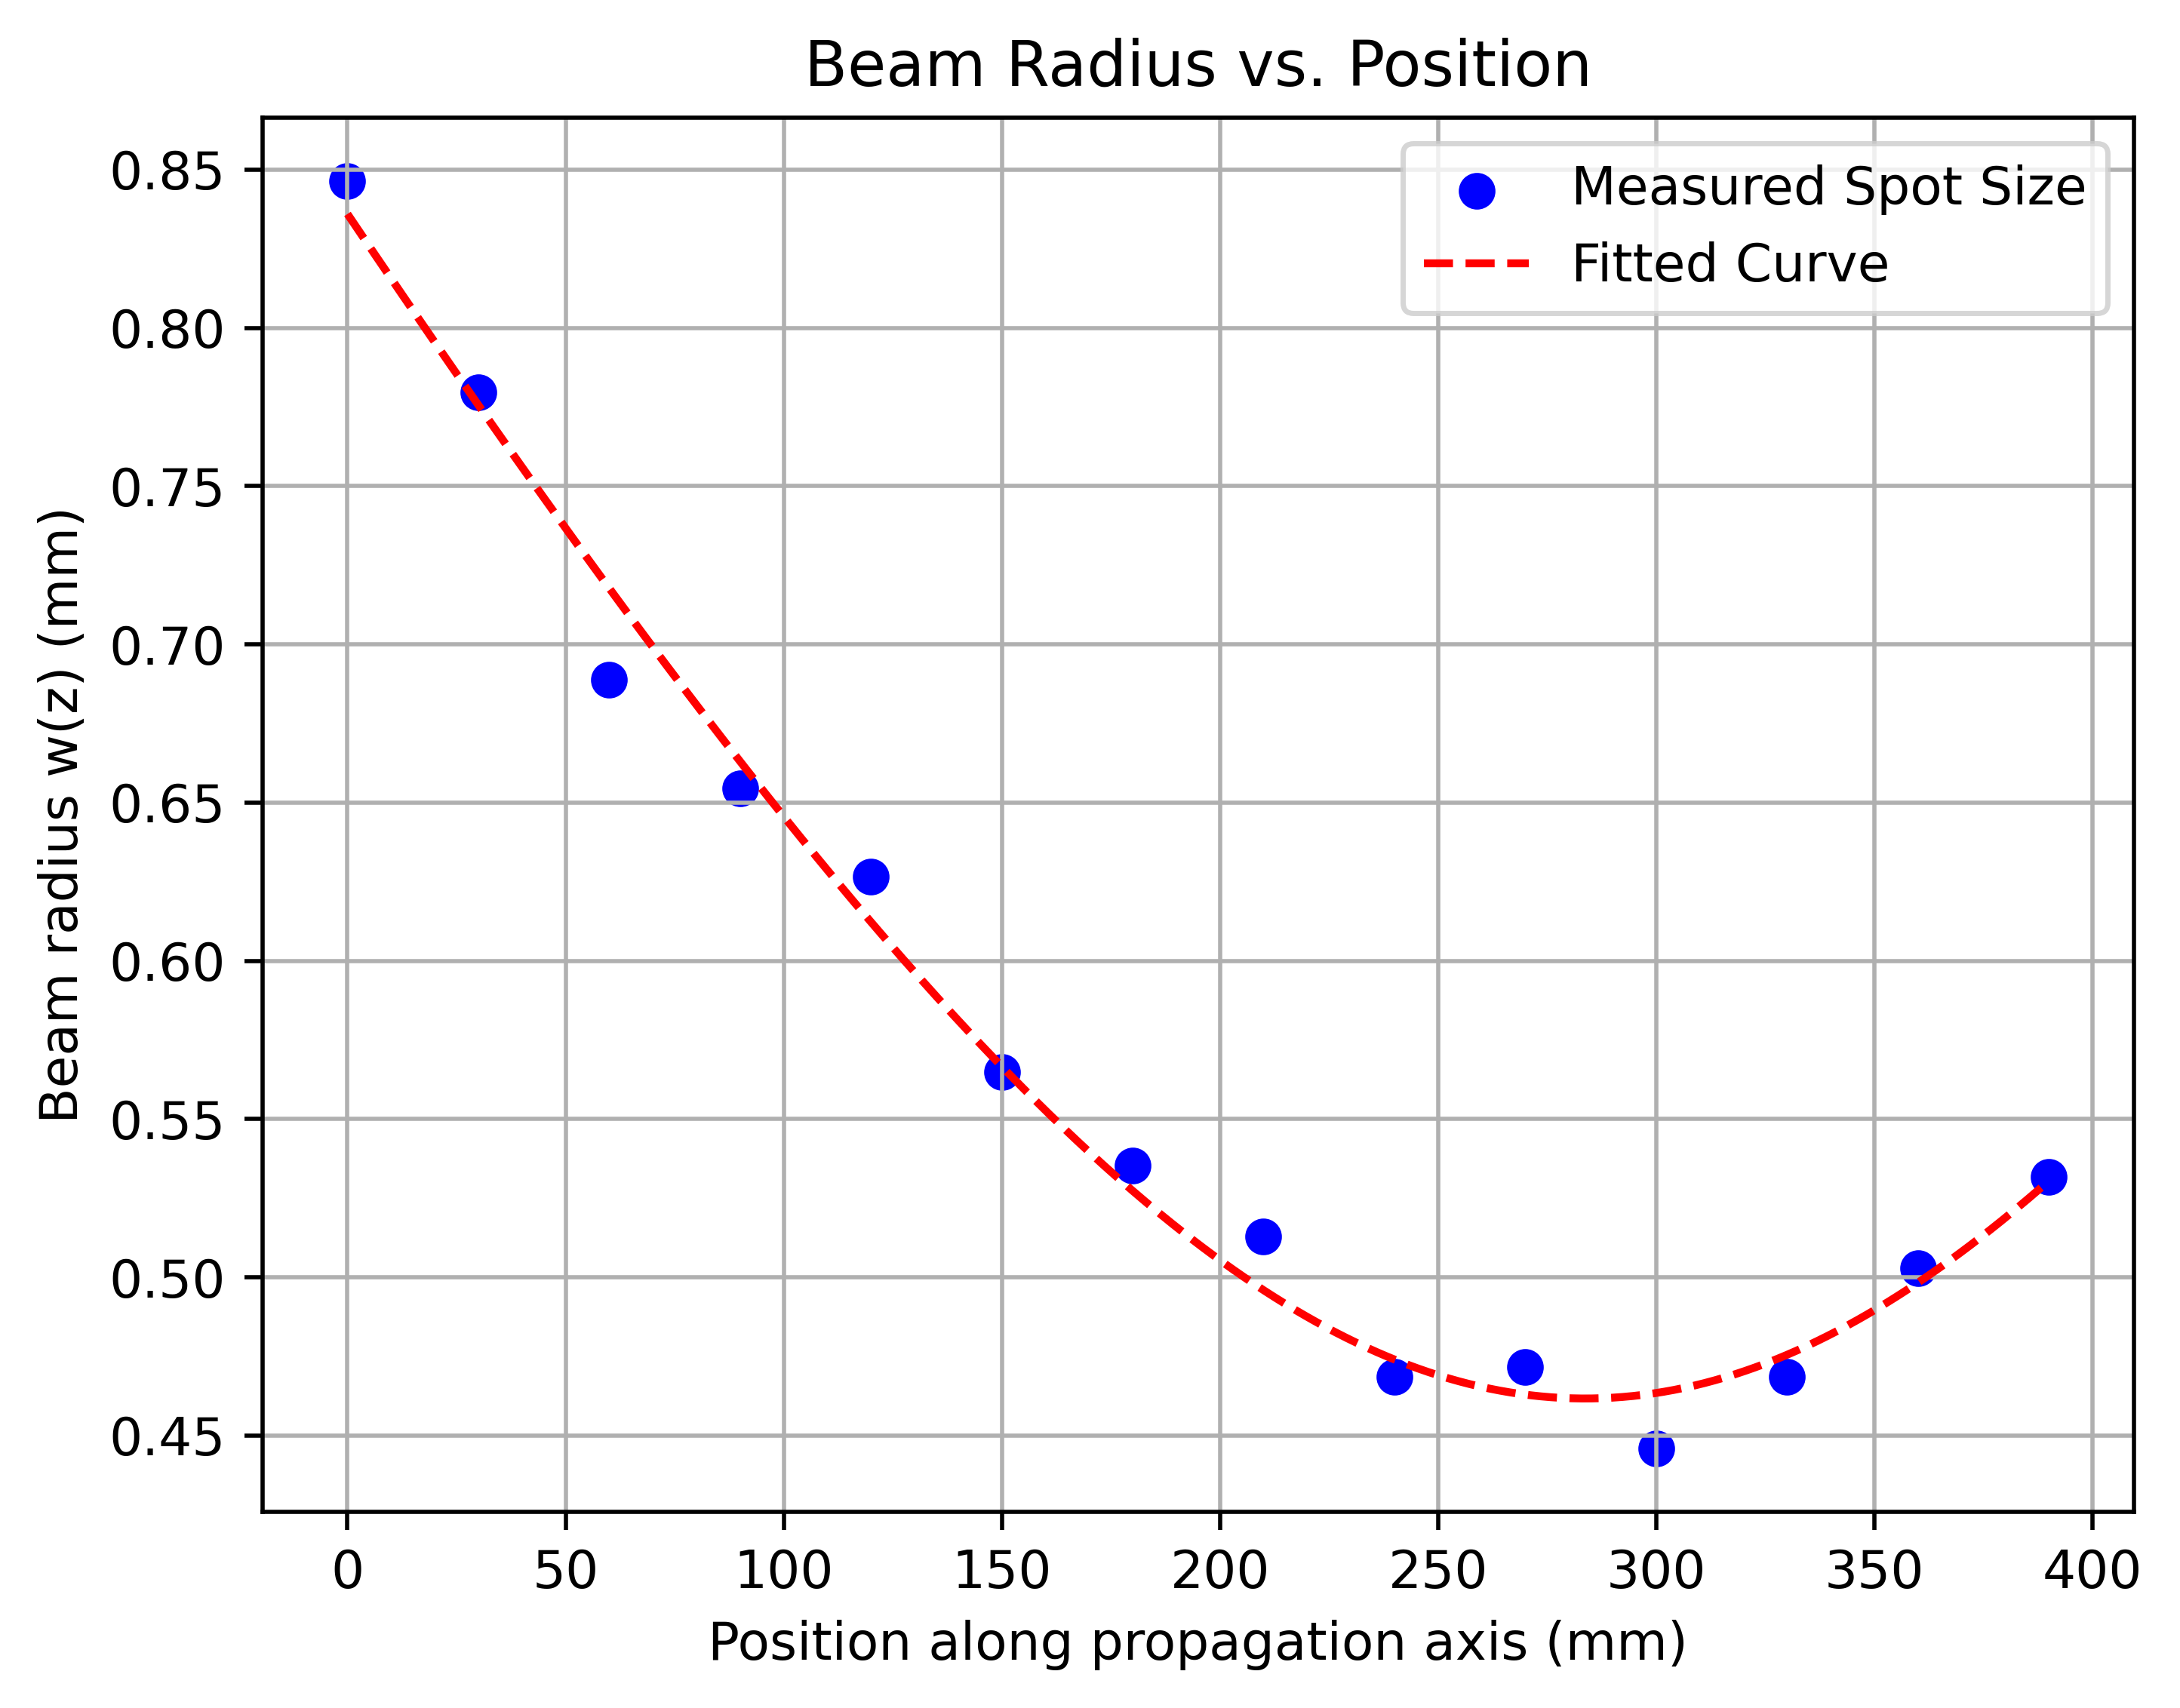
\includegraphics[width=0.6\linewidth]{images/APL1_8_exp3_analysis}
		\caption{高斯光束参数计算及数据点拟合}
		\label{fig:apl18exp3analysis}
	\end{figure}
	
	\item 高斯光束传播特性分析
	\begin{enumerate}
		\item 按实验3的方法,我们首先对加装透镜的测量结果进行数据处理。结果如\cref{tab:exp4-a-lens}和\cref{fig:apl18exp4analysislens}所示。
		
		\begin{table}[h!]
			\centering
			\renewcommand{\arraystretch}{1.5} % 调整行高
			\caption{Beam Parameters (exp4 with lens)}
			\label{tab:exp4-a-lens}
			\begin{tabular}{|c|c|}
				\hline
				\textbf{Parameter} & \textbf{Value} \\ \hline
				Beam Waist Position ($z_0$) & 277.78 mm \\ \hline
				Beam Waist Radius ($\omega_0$) & 0.4458 mm \\ \hline
				Divergence Angle ($\theta$) & 0.002268 rad \\ \hline
				Rayleigh Length ($Z_0$) & 196.57 mm \\ \hline
			\end{tabular}
		\end{table}
		
		\begin{figure}[h!]
			\centering
			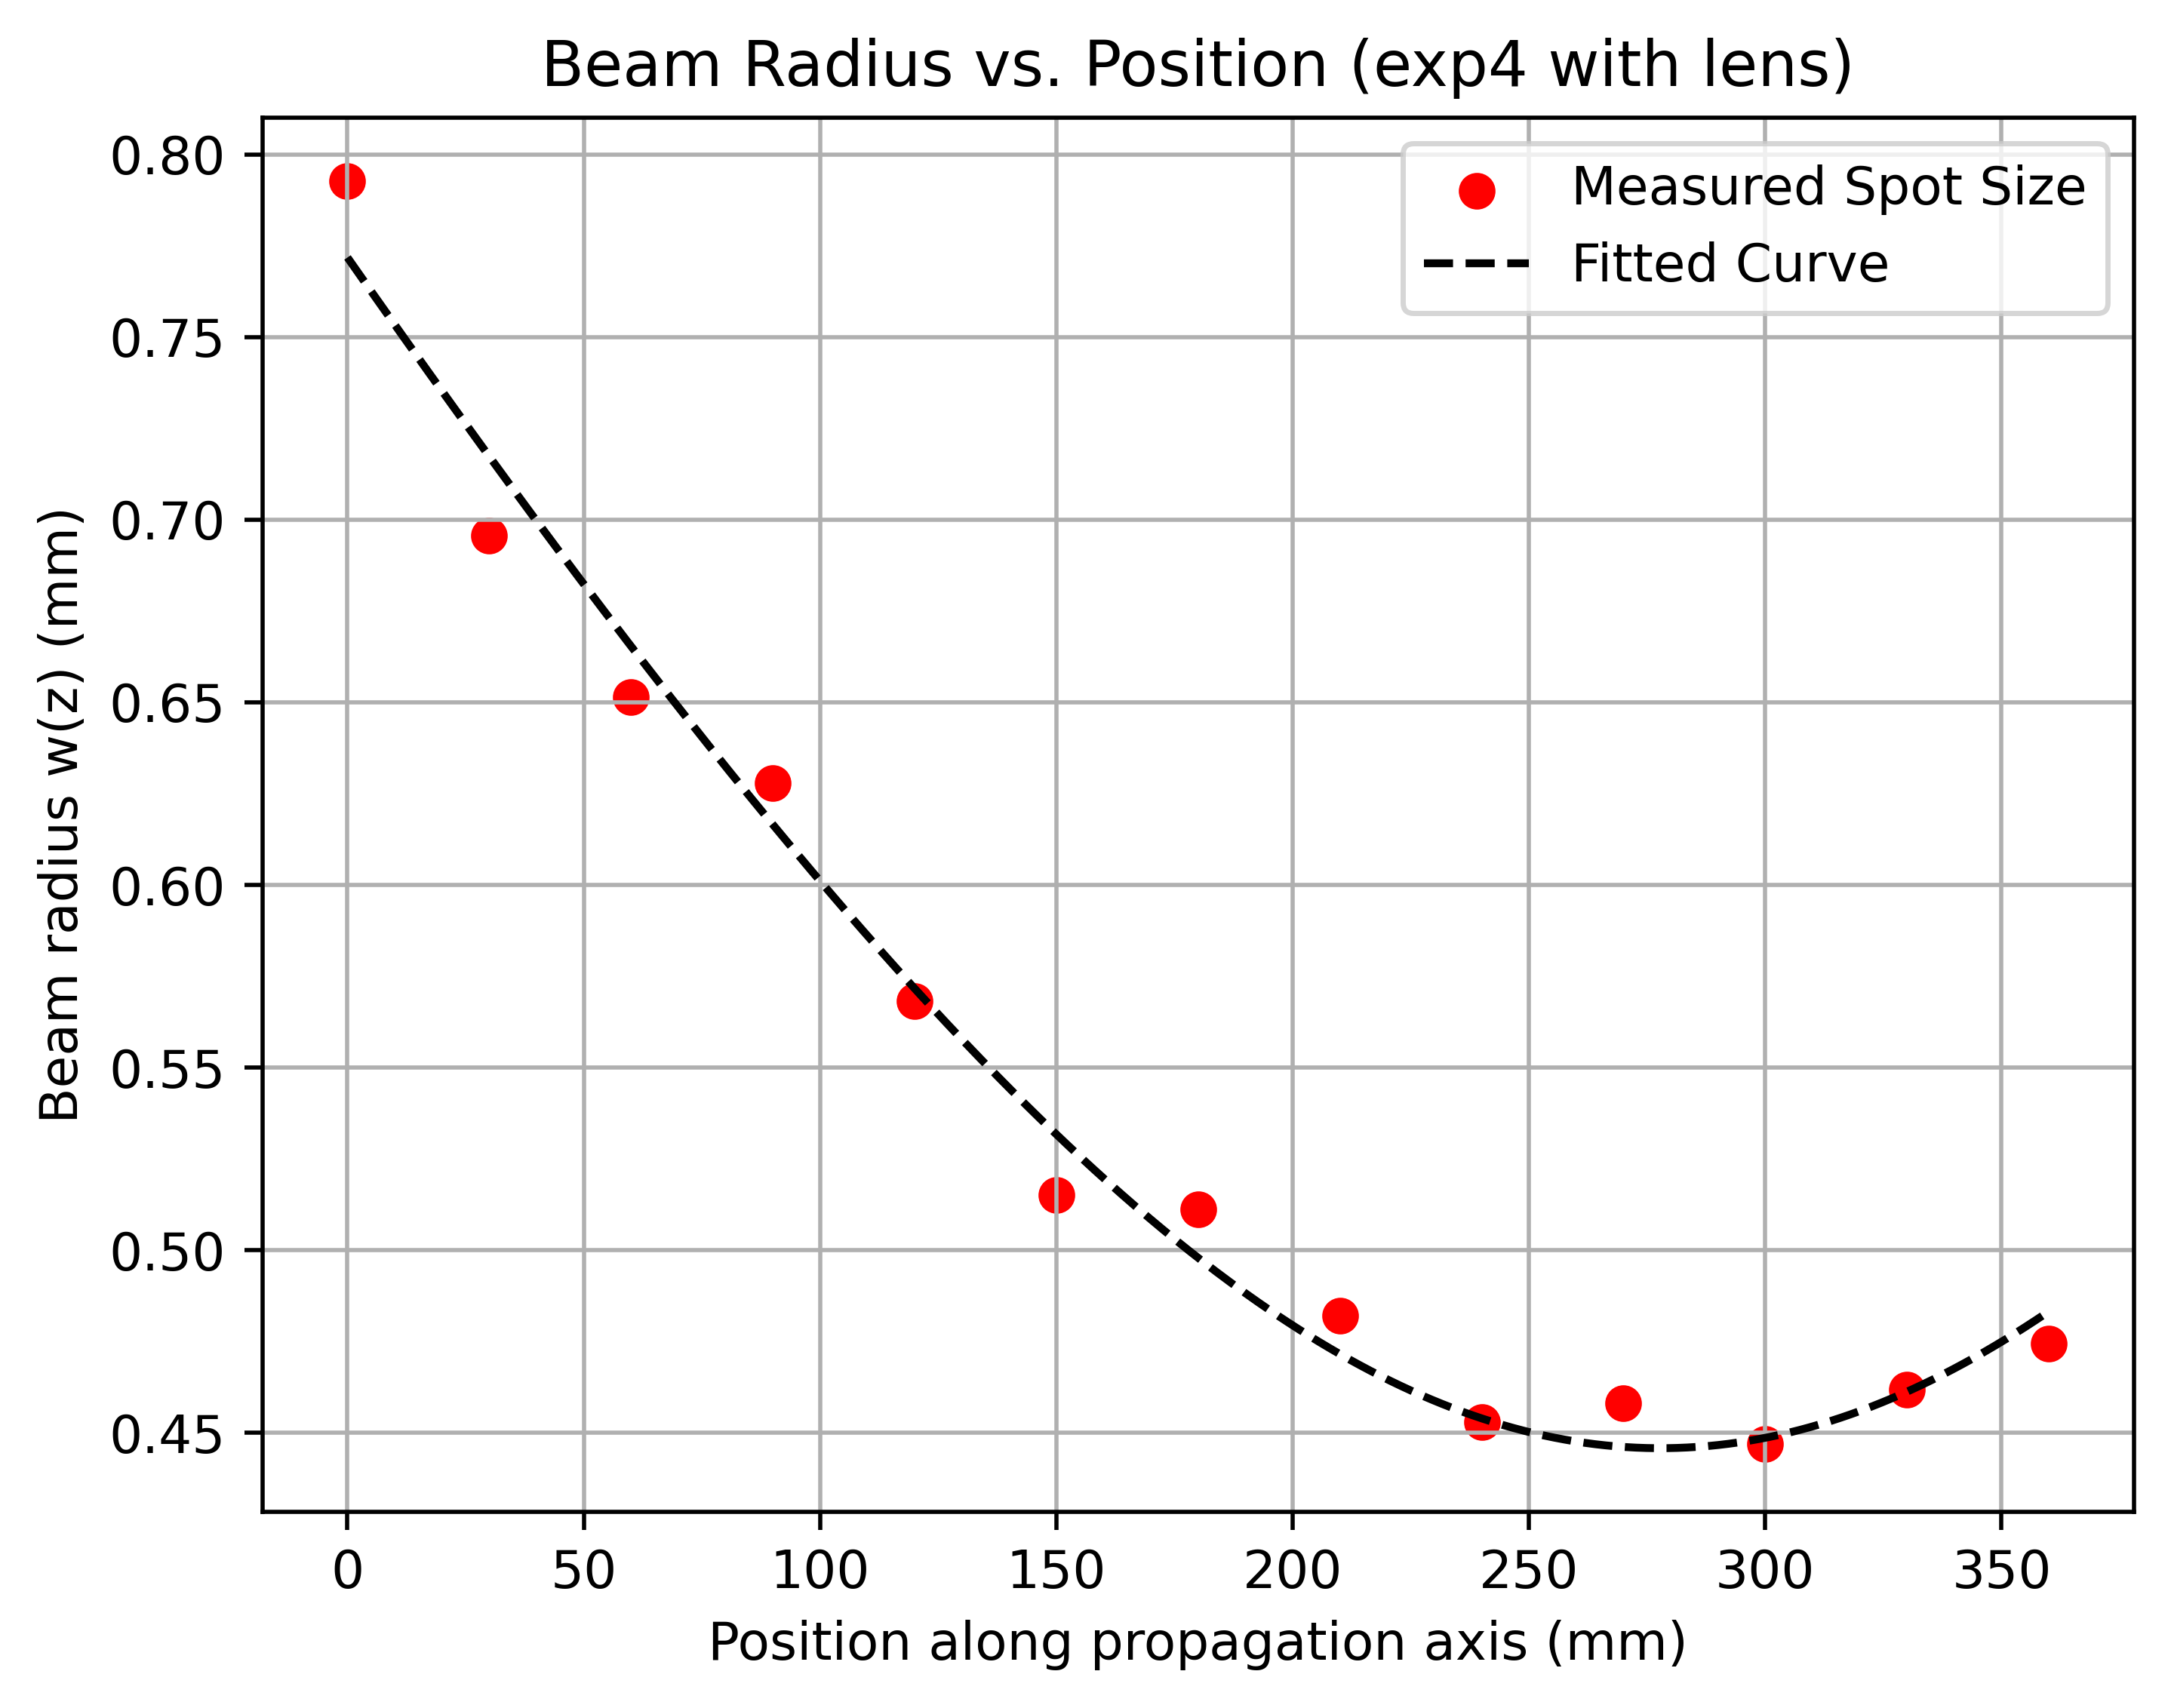
\includegraphics[width=0.6\linewidth]{images/APL1_8_exp4_analysis_lens}
			\caption{高斯光束传播特性分析:数据点拟合(加装透镜)}
			\label{fig:apl18exp4analysislens}
		\end{figure}
		
		\item 接下来考虑对无透镜情况进行数据处理,首先还是按照前面的方法,得到了如\cref{tab:exp4-a-nolens}和\cref{fig:apl18exp4analysisnolens1}所示结果。
		
		\begin{table}[h!]
			\centering
			\renewcommand{\arraystretch}{1.5} % 调整行高
			\caption{Beam Parameters (exp4 with no lens)}
			\label{tab:exp4-a-nolens}
			\begin{tabular}{|c|c|}
				\hline
				\textbf{Parameter} & \textbf{Value} \\ \hline
				Beam Waist Position ($z_0$) & 678.91 mm \\ \hline
				Beam Waist Radius ($\omega_0$) & 0.3035 mm \\ \hline
				Divergence Angle ($\theta$) & 0.002068 rad \\ \hline
				Rayleigh Length ($Z_0$) & 146.76 mm \\ \hline
			\end{tabular}
		\end{table}
		
		\begin{figure}[h!]
			\centering
			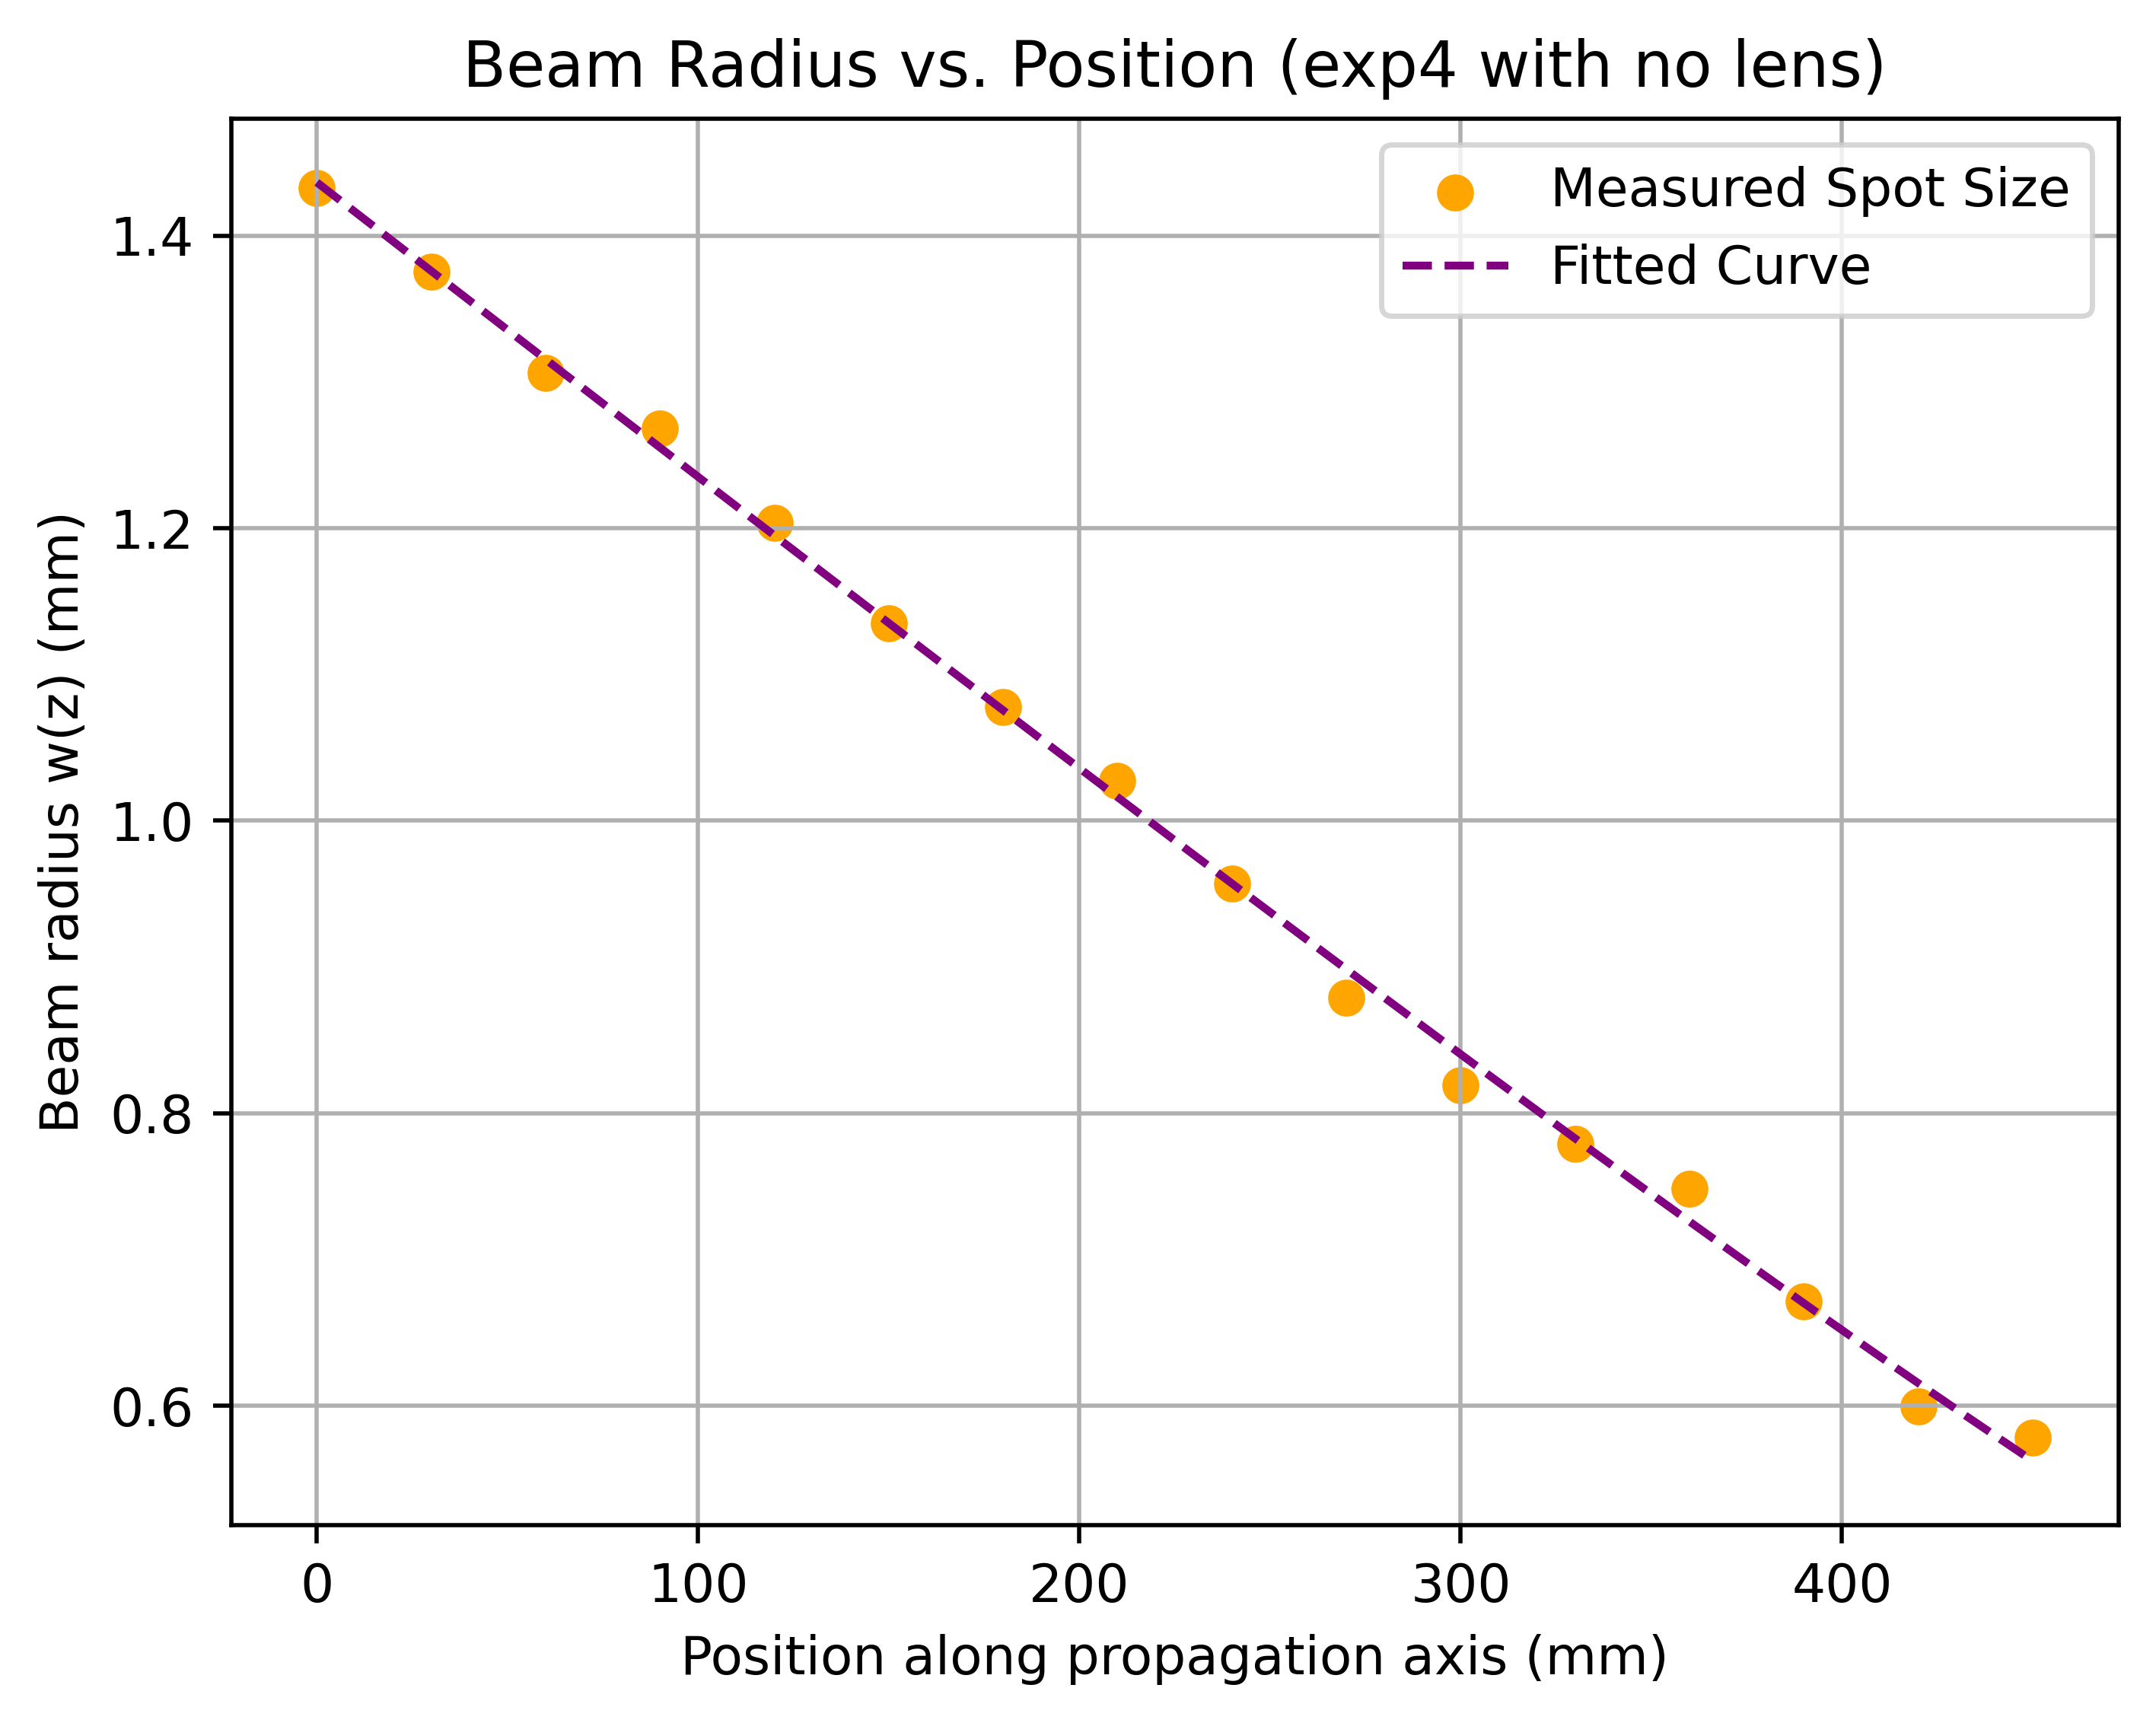
\includegraphics[width=0.6\linewidth]{images/APL1_8_exp4_analysis_nolens_1}
			\caption{高斯光束传播特性分析:数据点拟合(双曲线,不装透镜)}
			\label{fig:apl18exp4analysisnolens1}
		\end{figure}
		
		考虑到从拟合曲线上看,它几乎已经成了一条直线,因此我们考虑线性拟合的方案(相当于在计算双曲线的渐近线),结果如\cref{fig:apl18exp4analysisnolens2}所示。
		
		\begin{figure}[h!]
			\centering
			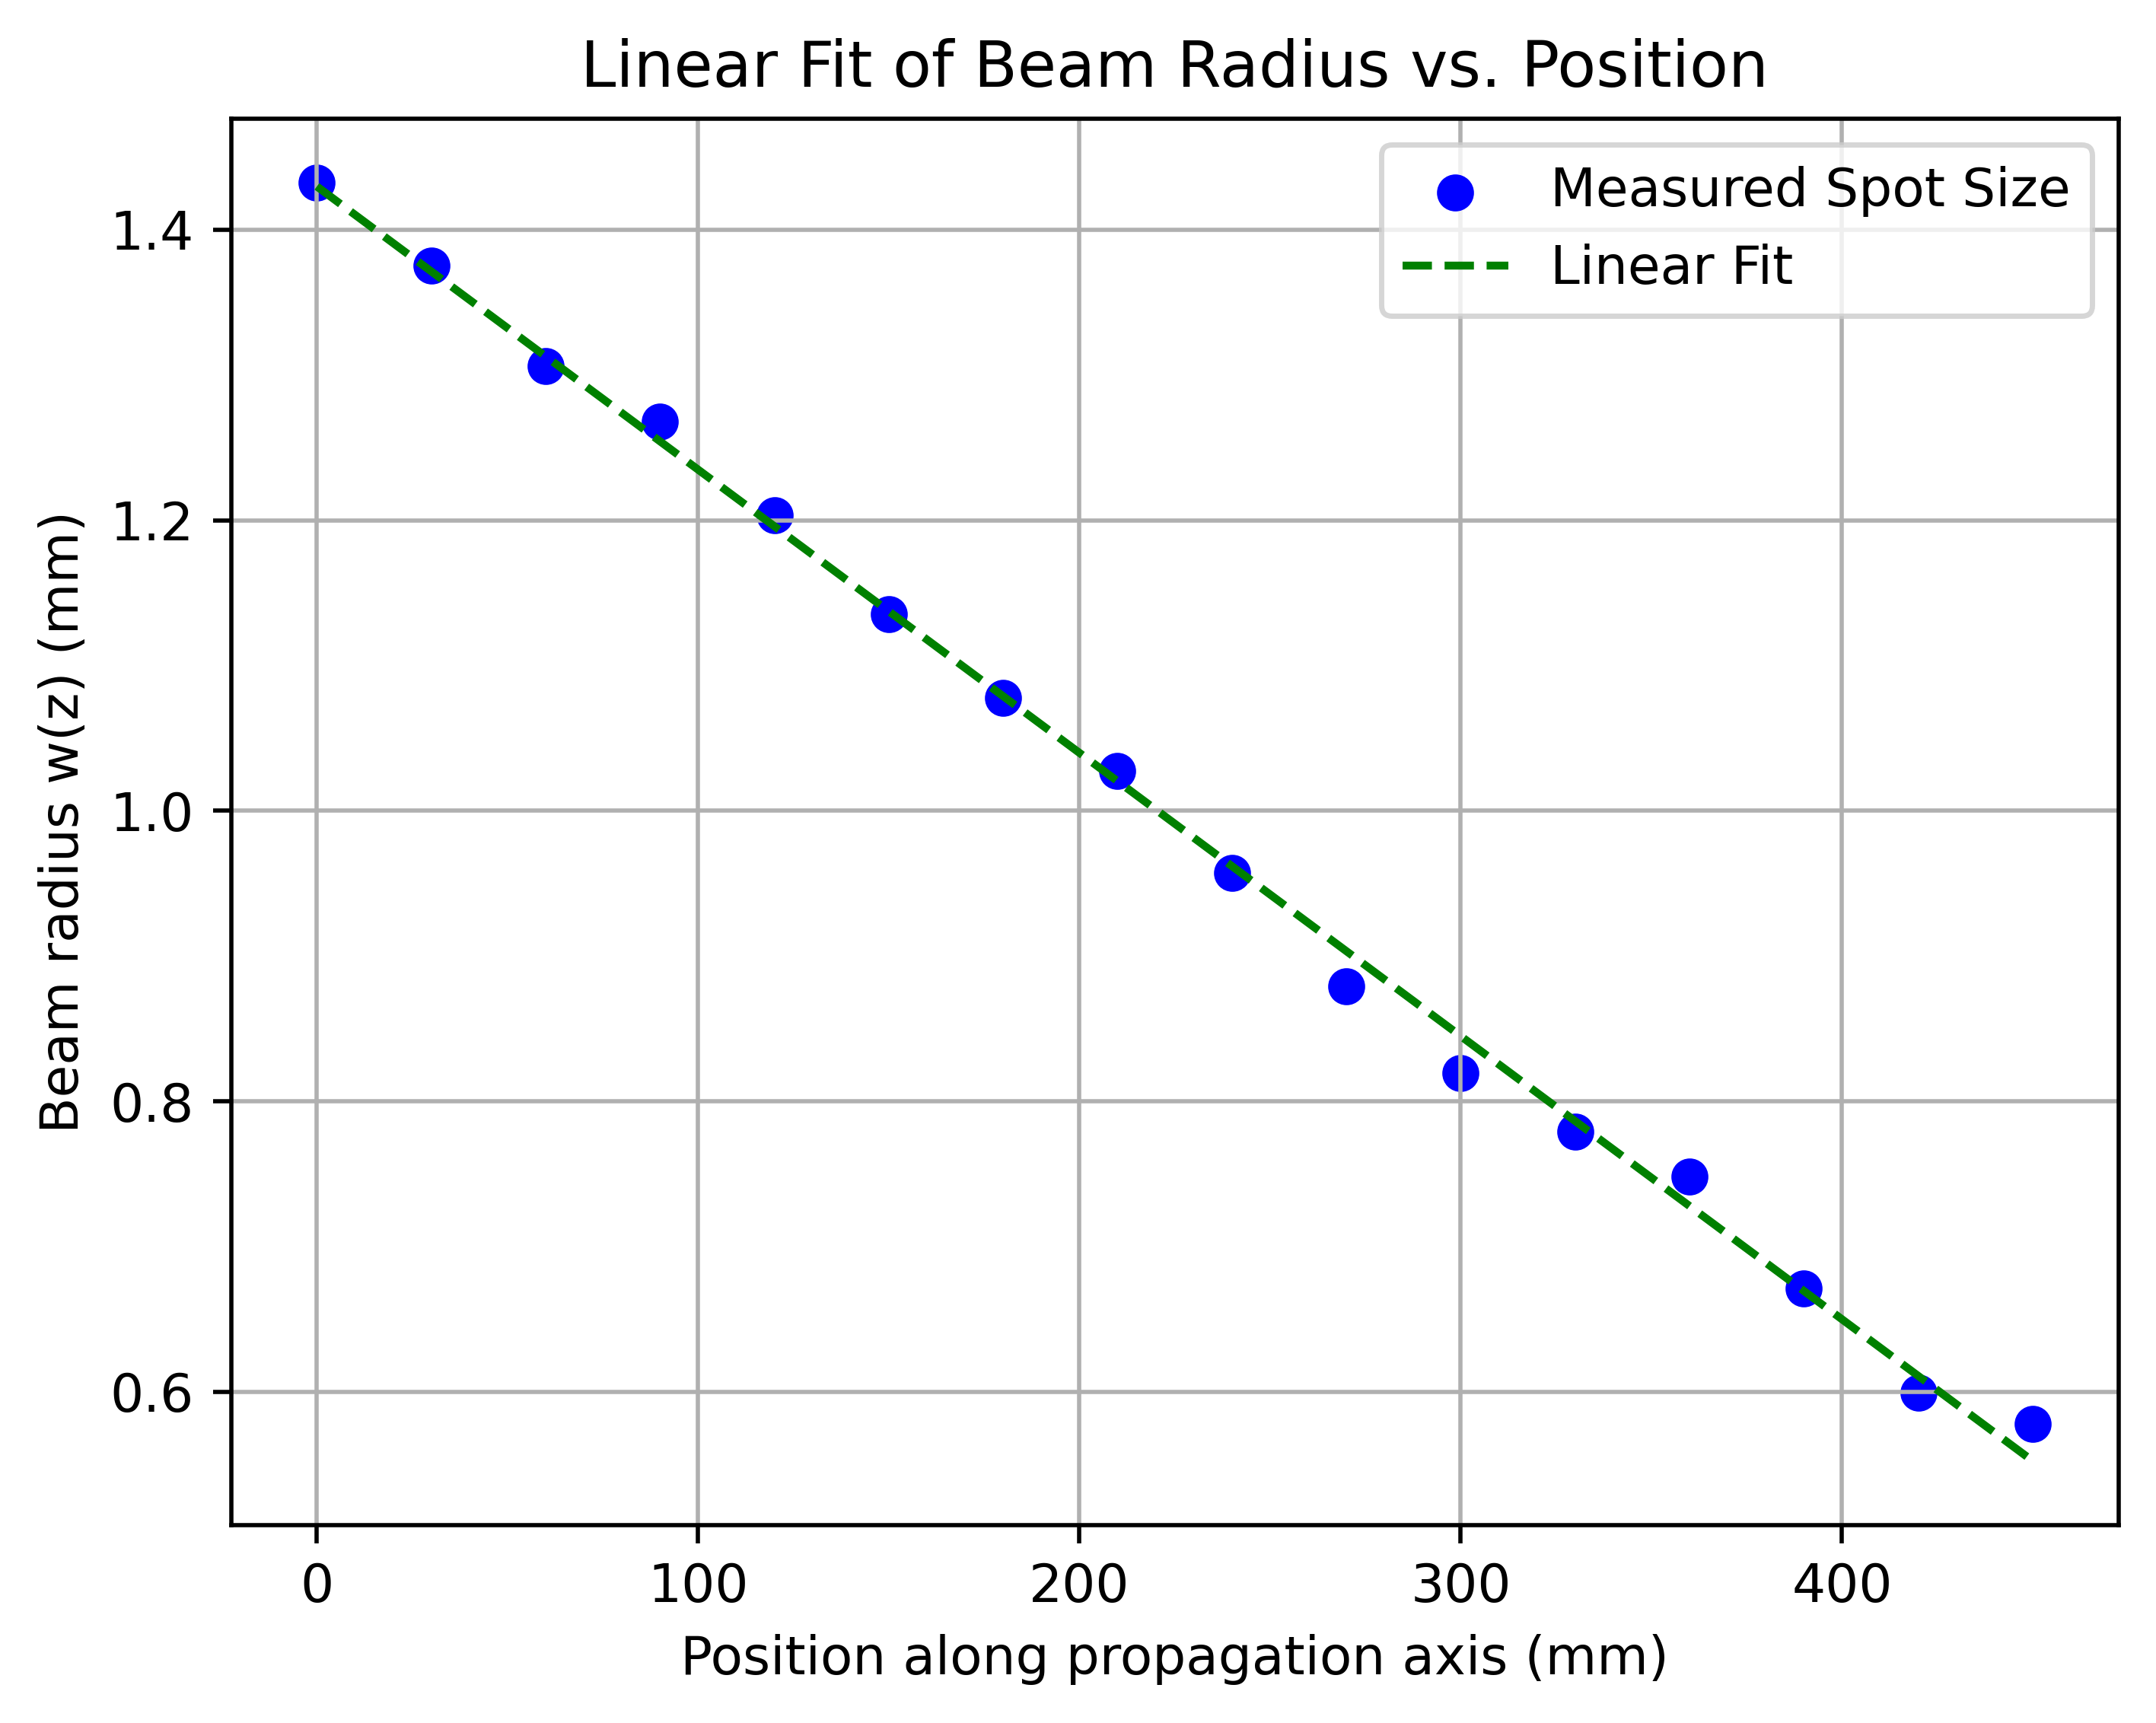
\includegraphics[width=0.6\linewidth]{images/APL1_8_exp4_analysis_nolens_2}
			\caption{高斯光束传播特性分析:数据点拟合(直线,不装透镜)}
			\label{fig:apl18exp4analysisnolens2}
		\end{figure}
		
		根据线性拟合得到的斜率(\(m\)),可以利用高斯光束的远场发散角公式来反推光束的其他参数,如束腰半径(\(\omega_0\))和瑞利长度(\(z_R\))。
		
		对于高斯光束,远场发散角(\(\theta\))可以表示为:
		\[
		\theta = \frac{\lambda}{\pi \omega_0}
		\]
		
		在远场区域,光束半径 \(w(z)\) 随距离 \(z\) 的变化近似线性关系,因此拟合斜率 \(m\) 可以直接表示发散角:
		\[
		m = \frac{d w(z)}{d z} = \theta
		\]
		
		通过拟合得到的 \(m\),我们得到了远场发散角 \(\theta\)。
		
		通过远场发散角公式,可以反推束腰半径 \(\omega_0\):
		\[
		\omega_0 = \frac{\lambda}{\pi m}
		\]
		
		瑞利长度 \(z_R\) 表示光束在束腰处至光斑面积增大一倍的位置之间的距离。可以通过以下公式计算瑞利长度:
		\[
		z_R = \frac{\pi \omega_0^2}{\lambda}
		\]
		
		根据远场区域的线性拟合结果,可以进一步推导高斯光束的束腰位置(即光束半径最小的位置,记为 \(z_0\))。该位置是光束半径随距离 \(z\) 增大趋势的起点,即当光束逐渐发散时的起点。
		
		在高斯光束模型中,光束半径 \(w(z)\) 随传播距离 \(z\) 的变化公式为:
		\[
		w(z) = \omega_0 \sqrt{1 + \left(\frac{z - z_0}{z_R}\right)^2}
		\]
		
		在远场区域,即 \(z \gg z_R\) 时,\(w(z)\) 可以近似为线性关系:
		\[
		w(z) \approx \omega_0 + \theta (z - z_0)
		\]
		
		将其整理为:
		\[
		w(z) \approx \theta z + \left(\omega_0 - \theta z_0\right)
		\]
		
		这实际上是一个线性方程,符合我们通过实验数据拟合得到的形式:
		\[
		w(z) = m \cdot z + c
		\]
		
		由此可以得到两个匹配条件:
		\[
		m = \theta
		\]
		\[
		c = \omega_0 - \theta z_0
		\]
		
		根据上述公式,可以解出束腰位置 \(z_0\):
		\[
		z_0 = \frac{\omega_0 - c}{\theta}
		\]
		
		综上所述,我们得到如\cref{tab:exp4-a-nolens-linear}所示结果。
		
		\begin{table}[h!]
			\centering
			\caption{激光束参数测量结果}
			\label{tab:exp4-a-nolens-linear}
			\begin{tabular}{|c|c|}
				\hline
				\textbf{参数}                     & \textbf{值} \\ \hline
				Slope ($m$)                       & -0.001950  \\ \hline
				Intercept ($c$)                   & 1.429826   \\ \hline
				$R$-squared                       & 0.9975     \\ \hline
				Mean Squared Error (MSE)          & 0.000182   \\ \hline
				Beam Waist Radius ($\omega_0$)    & 0.1033 mm  \\ \hline
				Rayleigh Length ($z_R$)           & 0.0530 mm  \\ \hline
				Beam Waist Position ($z_0$) - 双曲线近似  & 680.2766 mm \\ \hline
				Beam Waist Position ($z_0$) - 渐近线 & 733.2494 mm \\ \hline
			\end{tabular}
		\end{table}
		
		\item 利用上述结果,我们计算比对q参数,结果如\cref{tab:exp4-q}所示。
		
		\begin{table}[h!]
			\centering
			\caption{q参数数据}
			\label{tab:exp4-q}
			\begin{tabular}{|c|c|c|c|}
				\hline
				\textbf{拟合方法} & \textbf{透镜状态} & \textbf{实部} & \textbf{虚部} \\ \hline
				双曲线拟合 & 加装透镜出射光 & -162.22 & 196.57 \\ \hline
				双曲线拟合 & 未加装透镜入射光 & 238.91 & 146.76 \\ \hline
				双曲线拟合 & 变换后出射光 & -267.52 & 254.65 \\ \hline
				线性拟合双曲线近似 & 未加装透镜入射光 & 240.28 & 52.97 \\ \hline
				线性拟合双曲线近似 & 变换后出射光 & -563.81 & 478.49 \\ \hline
				线性拟合进近线近似 & 未加装透镜入射光 & 293.25 & 52.97 \\ \hline
				线性拟合进近线近似 & 变换后出射光 & -524.30 & 184.23 \\ \hline
			\end{tabular}
		\end{table}
		
	\end{enumerate}
	
\end{enumerate}

% 讨论
\subsubsection{Discussion}
\begin{enumerate}
	\item 关于谐振腔调节方法的讨论
	
	由戴鹏辉22344016主导,我们对谐振腔的调节作了如下总结:
	\begin{itemize}
		\item 调节方法:
		\begin{itemize}
			\item 按照实验装配图安装所有的器件。
			\item 使用台灯照亮十字叉丝板,叉丝线朝向半外腔激光器。
			\item 通过叉丝板中心小孔,目视氦氖激光器毛细腔,可看到一个蓝色的极亮斑和叉丝板的像。
			\item 通过调整后腔镜旋钮,将十字叉丝板的像的中心调整至与毛细管极亮斑重合。
			\item 反复调节,直至激光器发光。
		\end{itemize}
		
		\item 心得:
		\begin{itemize}
			\item 由于很难保证叉丝板与光路垂直,所以即是将叉丝板的像的中心调整至与毛细管亮斑重合,一般也很难使得激光发光。所以可尝试在亮斑周围四处调整。
			\item 操作时,两个旋钮同时调节。一个旋钮在原位缓慢的来回旋动或来回步进旋动,另一个旋钮在原位较快速的来回旋动。这就相当于镜片与管轴在基本垂直的位置上扫动,寻找最佳垂直位置,使之出光。
			\item 当激光器出光后,在仅调整后腔镜位置,不改变倾斜角度的情况下,激光器往往依然能出光;若不出光,仅需轻微调整后腔镜倾斜角度即可。
		\end{itemize}
	\end{itemize}
	
	\item 分析激光模式对光斑宽度的影响
	根据实验测量数据\cref{tab:exp2-1}、\cref{tab:exp2-2}和\cref{tab:exp2-3},分析单模和多模 He-Ne 激光在不同位置的光斑宽度,可以从水平宽度(\(a\) 轴)和垂直宽度(\(b\) 轴)两个方向进行对比,探讨激光模式对光斑宽度的影响。
	\begin{itemize}
		\item 单模 He-Ne 激光光斑宽度分析
		\begin{itemize}
			\item 在单模激光模式下,光束的发散性较小,光束的形状接近高斯分布,通常具有较小的光斑宽度,且随距离变化较为平缓。
			\item 单模激光器的光斑宽度随着测量位置的增加逐渐增大,这符合高斯光束在自由空间传播中的发散特性。
			\item 水平宽度和垂直宽度的变化较小,但可以观察到垂直宽度的数值比水平宽度略大,这表明光束在不同方向上的发散性有些微差异。
		\end{itemize}
		
		从单模激光的测量数据中可以看到:
		\begin{itemize}
			\item 水平宽度(\(a\) 轴)从 60 cm 位置的 0.5505 mm 增至 90 cm 位置的 0.9410 mm,增幅较为均匀。
			\item 垂直宽度(\(b\) 轴)从 60 cm 位置的 0.6517 mm 增至 90 cm 位置的 1.2908 mm,增加幅度与水平宽度相近,表明单模激光的光斑形状在传播过程中相对保持稳定。
		\end{itemize}
		
		\item 多模 He-Ne 激光光斑宽度分析
		\begin{itemize}
			\item 多模激光束通常包含多个频率或空间模式,导致其光斑宽度较大,且发散性增强。
			\item 在测量位置增加时,多模激光的光斑宽度增长显著快于单模激光,尤其在水平宽度方向上,发散明显。
		\end{itemize}
		
		多模激光的数据分析表明:
		\begin{itemize}
			\item 水平宽度(\(a\) 轴)从 60 cm 位置的 1.0166 mm 增至 90 cm 位置的 2.0274 mm,增幅较大。
			\item 垂直宽度(\(b\) 轴)从 60 cm 位置的 0.7482 mm 增至 90 cm 位置的 1.4523 mm,相比水平宽度的增幅略小,但远高于单模激光的增幅。
		\end{itemize}
		
		\item 激光模式对光斑宽度的影响
		
		对比单模和多模激光的测量数据,可以总结出以下几点:
		
		\begin{enumerate}
			\item \textbf{发散性}:多模激光的发散性显著高于单模激光,这在远场区域尤为明显,表现为光斑宽度随距离显著增大。单模激光则保持较小的发散角,使得光束在传播过程中的光斑宽度增加较缓。
			\item \textbf{光束质量与相干性}:单模激光模式具有较好的光束质量,其高斯分布特性更明显,因此相干性和方向性更强;而多模激光包含多个横模和纵模,相干性和方向性相对较差,导致光斑宽度的扩散速度更快。
			\item \textbf{横截面形状}:多模激光在传播过程中光束形状变得更加不规则,而单模激光的光斑形状在传播中更加稳定,对称性较好。
		\end{enumerate}
		
		\item 结论
		
		激光模式对光斑宽度有显著影响。单模 He-Ne 激光在不同测量位置下的光斑宽度增加较小,且在横纵两个方向的发散相对稳定,符合高斯光束特性,展现出较好的光束质量。而多模 He-Ne 激光在测量位置增加时光斑宽度显著增加,尤其在水平方向上的发散更为显著,反映出多模激光束中不同模式间的干扰和相干性不足。
	\end{itemize}
	
	\item 评估高斯光束参数和高斯光束传播特性的测量结果
	
	该部分分析由\textbf{朱政鑫22344019}主导完成。
	
	在实验中,我们分别对无透镜和加透镜的 He-Ne 激光器光束参数进行了测量和拟合分析。实验主要关注激光发散角、光腰位置和光腰半径的变化,并对拟合结果的可靠性进行了评估。
	
	无透镜组的测量数据通过测量软件自带拟合功能以及手动拟合方法获得。测量数据包括多组发散角、光腰位置和光腰半径的拟合值,并在此基础上对加透镜后的光束参数进行了预测。
	通过无透镜测量数据的拟合得到发散角约为 0.3736 mrad,光腰位置约为 1253.17 mm,光腰半径为 1 mm。利用这些值计算了远场发散角、光腰位置和光腰半径的预测值。
	无透镜组的预测值与实验结果差异较大,仅有 1a 测量组的预测值与实验结果偏差在 50\% 内,其余测量组的预测结果均超出合理范围。大多数数据表明,预测结果和实际值存在显著误差,拟合值达到约束极限,导致数据的适用性和可靠性受到限制。
	无透镜组的拟合数据无法获得可靠的光束参数,所有拟合结果均存在明显偏差。结果表明,无透镜条件下的数据不支持可行的光束参数拟合,仅个别数据偏差在可接受范围内。
	
	加透镜组的测量数据同样来自测量软件自带拟合功能。测量的发散角、光腰位置和光腰半径在透镜位置 660 mm 和 670 mm 的条件下分别进行了测试。
	加透镜组的拟合结果相对更为稳定。测量数据显示出发散角、光腰位置和光腰半径变化较为合理,拟合得到的光束参数基本在实验预期范围内,且符合理论模型的预测。例如,实验三 a 和三 b 组的发散角为约 1.311 mrad,光腰位置和光腰半径分别为 283.75 mm 和 0.19 mm,拟合结果具有较高的可靠性。
	加透镜组数据的拟合结果符合理论预期,数据质量较高,适用于进一步分析。实验表明,加透镜后光束的发散角和光腰参数可以通过拟合数据较为准确地预测。
	
	通过手动拟合得到的发散角、光腰位置和光腰半径的计算结果与软件拟合结果存在一定偏差。实验手动测量值与拟合值的残差较大,表明手动拟合结果的精确度有限,但仍能够提供关于光束特性的一些基本信息。优化后的发散角为 0.3736 mrad,光腰位置为 1253.17 mm,光腰半径为 1 mm,反映出激光发散角和光腰位置在无透镜情况下难以准确预测。
	
	总体来看,加透镜条件下的测量数据可靠性较高,拟合结果与实际光束特性相符,可以用于光束传播特性分析。而无透镜组的数据拟合结果偏差较大,未能提供可靠的光束参数预测。建议进一步优化无透镜测量的实验方案,增加数据点以提高拟合准确性。
	
	\begin{figure}[h!]
		\centering
		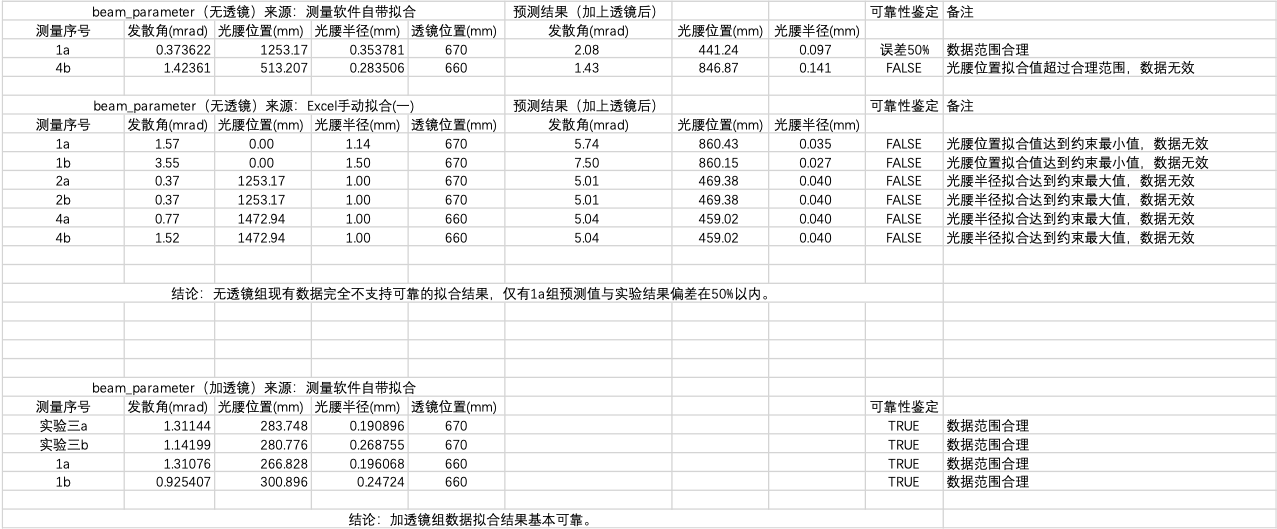
\includegraphics[width=0.7\linewidth]{images/APL1_8_exp4_analysis_zzx3}
		\caption{最终结论与结果评定}
		\label{fig:apl18exp4analysiszzx3}
	\end{figure}
	
	\begin{figure}[h!]
		\centering
		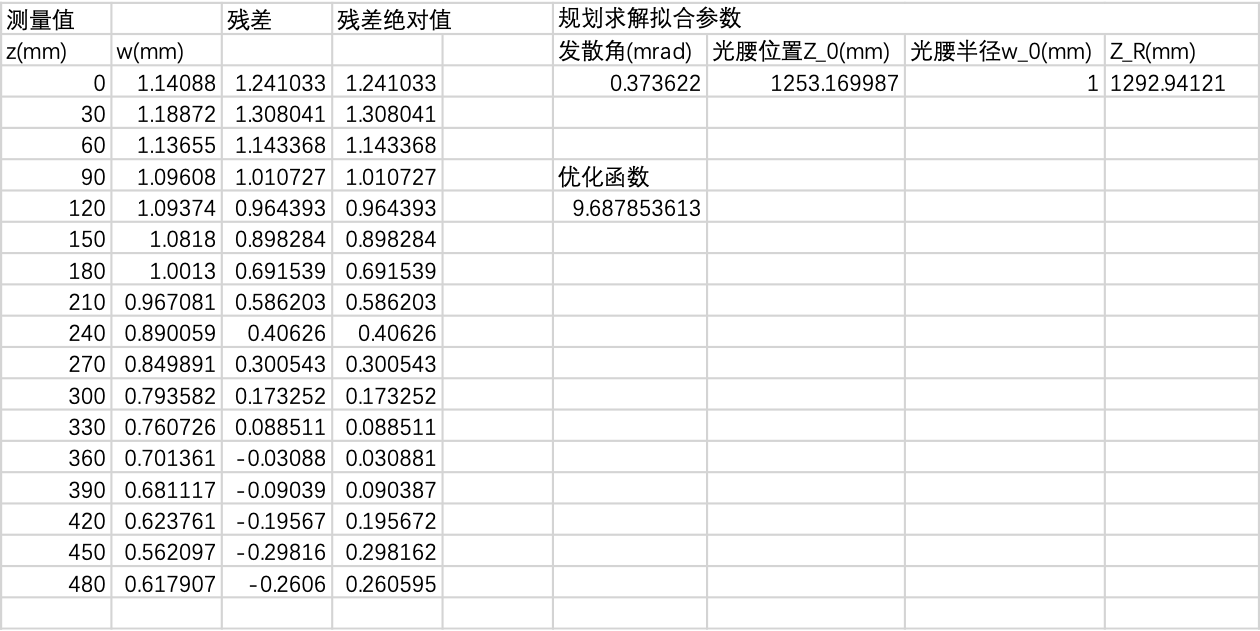
\includegraphics[width=0.7\linewidth]{images/APL1_8_exp4_analysis_zzx1}
		\caption{初步计算}
		\label{fig:apl18exp4analysiszzx1}
	\end{figure}
	
	\begin{figure}[h!]
		\centering
		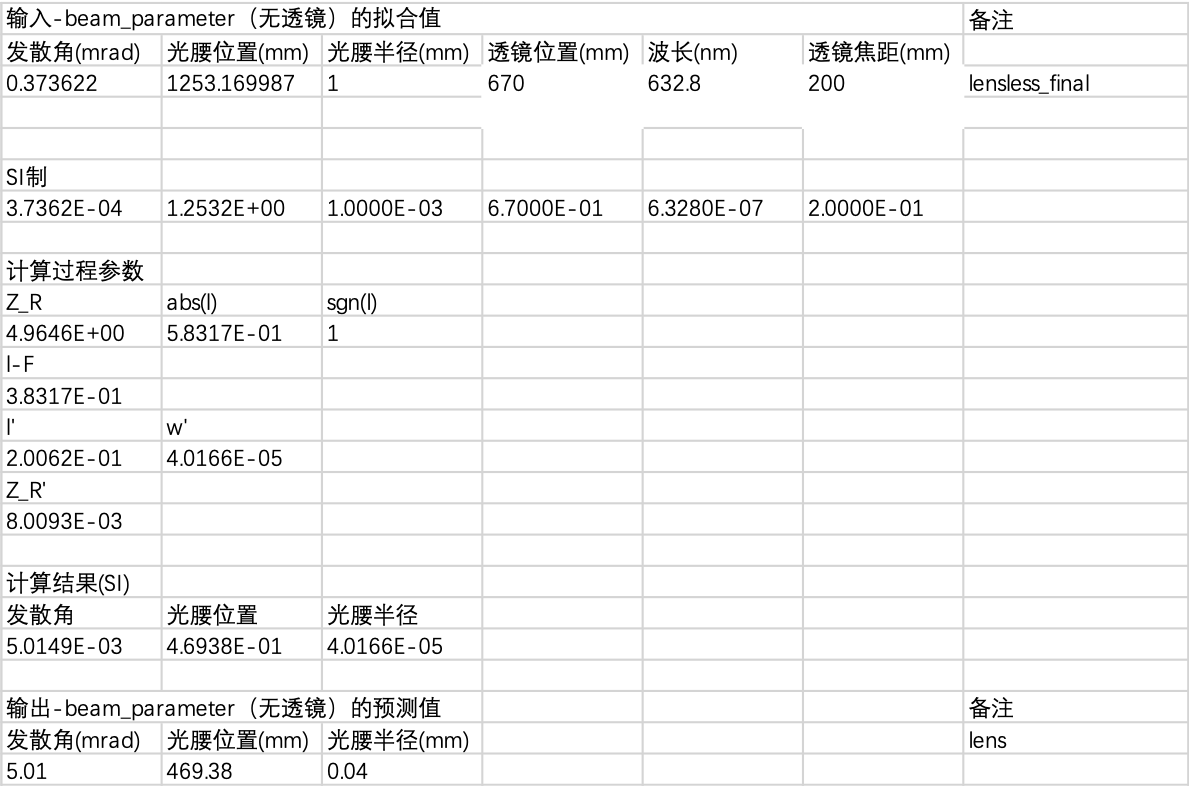
\includegraphics[width=0.7\linewidth]{images/APL1_8_exp4_analysis_zzx2}
		\caption{手动拟合}
		\label{fig:apl18exp4analysiszzx2}
	\end{figure}
	
	\item 更多讨论详见\textbf{实验后思考题}。
\end{enumerate}

%% 总结
%\subsubsection{Conclusion}
%\begin{itemize}
%	\item 
%\end{itemize}


%---------------------------------------------------------------------
% 实验后思考题
\subsection{Reflections after Experiment}

%思考题1
\begin{question}
	氦氖激光器直接输出的高斯光束的光腰位置在那里?光腰位置是否位于激光器的输出口?
\end{question}
氦氖激光器直接输出的高斯光束的光腰位置并不一定位于激光器的输出口,而是与激光器的光学设计和内部结构密切相关。光腰位置 \(z_0\) 是指光束达到最小半径的位置,它取决于激光器内部光学谐振腔的长度和配置。因此,需要通过实际测量和数据分析来确定光腰位置。

在无透镜情况下(即激光器直接输出高斯光束的情形),通过实验测量和数据拟合得出以下结果:
\begin{itemize}
	\item 无透镜条件下光腰位置 \( z_0 \) 被测量为 \textbf{678.91 mm}(见\cref{tab:exp4-a-nolens}),而线性拟合的近似方法则得到了略为不同的光腰位置 \textbf{733.25 mm}。
	\item 这两个结果都表明光腰位置远离激光器的输出口。
\end{itemize}

如果光腰位于激光器的输出口,那么测量得到的光束半径 \( w(z) \) 应该在输出口处达到最小值,而在远离输出口的方向上逐渐增大。然而,从测量数据的光束半径变化趋势可以看出,激光束在离开输出口后的某一位置才逐渐收敛至最小值,即光腰位置在激光器输出口的外部。

根据高斯光束的传播特性,当光束离开谐振腔后,会沿传播方向逐渐收敛,直至到达光束束腰位置。此后光束开始发散。氦氖激光器的谐振腔通常设计为稳定腔型,但其束腰位置会受到谐振腔反射镜曲率和腔长的影响,可能位于激光器内部的某个位置,也可能在输出口之外。

实验结果表明无透镜情况下的光腰半径 \( \omega_0 = 0.3035 \) mm 和光腰位置 \( z_0 = 678.91 \) mm,这一光腰位置较远,表明激光束在离开输出口之后逐渐聚焦至该位置。这种情况在自由空间中的激光传播中是典型的:激光束在离开谐振腔后,由于没有聚焦光学元件的约束,光腰位置便出现在远离输出口的位置。

高斯光束在无透镜情况下的传播符合高斯光束模型。无透镜条件下的数据表明,氦氖激光器的直接输出光束的光腰位置并不位于输出口,而是在输出口之外的某一距离处,这与实验结果中光腰位置约 678.91 mm 一致。因此,我们可以合理得出结论:在无透镜情况下,氦氖激光器的光腰位置位于输出口之外的数百毫米处。

综上所述,通过实验数据和高斯光束理论的结合分析,可以确定氦氖激光器直接输出的光束光腰位置位于距离输出口较远的位置。


% 思考题2
\begin{question}
	对照透镜的 ABCD 矩阵, $q_{in}$ 与 $q_{out}$ 是否与矩阵变化理论结果吻合?
\end{question}
要分析 \( q_{in} \) 和 \( q_{out} \) 是否符合透镜的 ABCD 矩阵变换理论,我们首先需要理解透镜的 ABCD 矩阵在光束传播中的作用。对于一个光学系统的 ABCD 矩阵,可以利用复数 \( q \) 参数来描述高斯光束在透镜前后的变化。

对于焦距为 \( f \) 的薄透镜,ABCD 矩阵可以写为:
\[
\begin{pmatrix}
	A & B \\
	C & D
\end{pmatrix}
= 
\begin{pmatrix}
	1 & 0 \\
	-\frac{1}{f} & 1
\end{pmatrix}
\]

根据光学系统中 \( q \) 参数的传播关系,透镜前后的 \( q \) 参数的关系可以通过 ABCD 矩阵变换表示为:
\[
q_{out} = \frac{A q_{in} + B}{C q_{in} + D}
\]

由于 \( A = 1 \)、\( B = 0 \)、\( C = -1/f \)、\( D = 1 \),可以简化为:
\[
q_{out} = \frac{q_{in}}{1 - \frac{q_{in}}{f}}
\]
其中,\( q \) 参数本身是复数,表示为:
\[
\frac{1}{q} = \frac{1}{R} - i\frac{\lambda}{\pi w^2}
\]

根据\cref{tab:exp4-q}中的数据,分别用双曲线拟合和线性拟合得到了不同状态下的 \( q \) 参数。第一组(即第一行数据)是直接测量的 \( q_{out} \),其余奇数序号的数据为计算得到的 \( q_{in} \) 值,然后利用透镜的 ABCD 矩阵进行变换得出的 \( q_{out} \) 值。
直接测量的 \( q_{out} \):在“加装透镜出射光”的第一组数据中,测量得到的 \( q_{out} \) 实部和虚部分别为 -162.22 和 196.57。这一数据反映了经过透镜后的光束特性,光束经过透镜聚焦,导致了 \( q_{out} \) 的实部为负,表明光束聚焦点距离透镜一定距离。
不同拟合方法得到的 \( q_{in} \) 及其矩阵变换后的 \( q_{out} \):我们观察不同方法算出的 \( q_{in} \)(未加装透镜入射光)值及其矩阵变换后的 \( q_{out} \) 值。这些方法(如双曲线拟合、线性拟合双曲线近似等)给出的结果显示出较大差异:
例如,双曲线拟合得到的 \( q_{in} \) 为 \( 238.91 + 146.76i \),经过矩阵变换后计算出的 \( q_{out} \) 为 \( -267.52 + 254.65i \),但与实际测量值 \( -162.22 + 196.57i \) 存在一定差异。

线性拟合双曲线近似和渐近线近似得到的 \( q_{in} \) 分别为 \( 240.28 + 52.97i \) 和 \( 293.25 + 52.97i \),经过透镜变换后的 \( q_{out} \) 也与直接测量值有明显差距(如 \( -563.81 + 478.49i \) 和 \( -524.30 + 184.23i \))。
从上述数据来看,利用不同方法计算的 \( q_{in} \) 经矩阵变换后的 \( q_{out} \) 与直接测量的 \( q_{out} \) 存在较大差异。理论上,通过 ABCD 矩阵变换后 \( q_{in} \) 应与实际的 \( q_{out} \) 保持一致,但实验结果中,变换后的 \( q_{out} \) 值的实部和虚部并未完全吻合。这种差异可能源于以下几个因素:
不同拟合方法(如双曲线拟合、线性拟合)在计算 \( q_{in} \) 时会引入不同程度的误差。特别是对于非线性分布的拟合,如果使用线性拟合方法,可能会低估或高估光束参数,从而影响 \( q_{in} \) 的计算精度;
在实验过程中,测量设备的精度、透镜位置的误差、激光光束的微小偏移等均可能导致实际测量的 \( q_{out} \) 偏离理论值;
实验中的光束可能不是理想的 TEM\(_{00}\) 模式高斯光束,而是有一定的光束质量因子 \( M² \),导致在透镜聚焦后,光束的发散角、光腰位置等与理想高斯光束有所偏差,从而影响 \( q \) 参数的变化。

综上所述,通过不同方法计算的 \( q_{in} \) 经 ABCD 矩阵变换后的 \( q_{out} \) 与实际测量的 \( q_{out} \) 存在明显差异。理论上,这些 \( q \) 参数应该在透镜的 ABCD 矩阵作用下转换一致,但实验中的差异表明,拟合方法和实验误差可能影响了结果的准确性。


% 思考题3
\begin{question}
	根据实验数据,光束通过透镜后,光腰是否位于透镜的焦点位置?请解释实验现象。
\end{question}
根据实验数据,光束在通过透镜后,光腰并不位于透镜的焦点位置。

从实验结果中,我们观察到:根据表格数据(\cref{tab:exp4-a-lens}),加装透镜后光束的光腰位置 \( z_0 \) 约为 277.78 mm,而透镜的位置在 670 mm。透镜的焦距为 \( f = 200 \) mm,那么如果光腰位于透镜焦点位置,则应该出现在 200 mm 处。然而,实验数据显示的光腰位置约为 277.78 mm,比透镜焦点更远。

对于理想的高斯光束,当其经过焦距为 \( f \) 的透镜时,光腰位置理论上应位于透镜焦点位置。但是,在实际实验中,光束通过透镜后的光腰位置可能偏离焦点,原因包括:在实验中,入射到透镜的光束并不一定是完全平行的。对于非理想平行光,透镜后的光束焦点会发生偏移,这会导致光腰位置不在透镜的焦点处;实际激光束可能偏离理想的 TEM\(_{00}\) 模式高斯光束,存在一定的发散性。实验中测得的 M² 因子表明,光束的发散特性并非理想高斯光束特性。M² 因子越大,光束的发散越明显,使得焦距位置有所偏离,导致光腰位置在焦点之外;透镜的实际焦距可能与标称值略有差异,这在一定程度上影响了光束的聚焦效果;光束半径和位置测量可能存在细微误差,尤其是在透镜前后位置的精确测量可能不够精确,导致对光腰位置的估算出现偏差。

总之,在本实验结果中,光束通过透镜后的光腰位置并不在透镜的焦点位置,而是出现在焦点稍远的位置。这一现象可能是由于激光束的非理想性(如 M² 因子偏离理想值)和实验误差所导致。
